% Drawing 141/01-8 -- folder 141, batch 01, archive page 10 (PDF page 11).
% Transcription: au-dessous, un cercle dont six arcs sont épaissis, alternant avec des arcs fins, et à l'intérieur une flèche courbe de rotation, montant vers la droite.
% Kind: circle with alternating heavy arcs and a rotation arrow. Method 2 (schematic redraw from the facsimile). Status: partial.
% Notes: The circle (an ellipse on the page, 31 by 30.3 units), six heavy arcs on it (a long one over the top right, one at the upper left, a long one on the left, one at the right, a short one below it at the lower right, one at the bottom right), separated by thin arcs, and inside the circle a curved arrow turning counter-clockwise, its head pointing up. Overlaid 2026-11-12 (Opus 5.5) on the 400 dpi colour crop and corrected: the circle was 2 units too low and 1 unit too small, so that the heavy arcs lay inside his outline; the circle and the arcs are redrawn on the page outline, each heavy arc between the directions of its two ends as read. Still differs: small ticks across the circle at the ends of some heavy arcs are not drawn. Redrawn 2026-11-12 (issue 128): to check again.
% Coordinates: 1 unit = 0.5 mm = 1/100 of the crop width (bbox in page fractions: [0.57, 0.575, 0.76, 0.685]).
% Redrawn by Claude (claude-fable-5-2), issue #128, 2026-11-12; not checked by a human; not compiled (no TeX in the session).
% Overlaid by Claude (claude-opus-5-5) 2026-11-12 (issue #128): rasterised from its own coordinates over the 400 dpi colour facsimile and corrected from it. Not compiled. Status: partial.
% Rights: reproduces part of the work -- behind RENDER_TRANSCRIPTS, never published by itself.
\documentclass[tikz,border=3pt]{standalone}
\usepackage{amsmath,amssymb}
\usetikzlibrary{patterns,arrows.meta}
\tikzset{pencil/.style={black!45}, struck/.style={black!35}, mpt/.style={circle,draw,inner sep=1.3pt}, pt/.style={circle,fill,inner sep=0.9pt}, opt/.style={circle,draw,fill=white,inner sep=1.1pt}}
\begin{document}
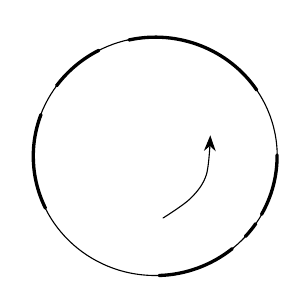
\begin{tikzpicture}[x=0.5mm,y=0.5mm,line cap=round,line join=round,font=\scriptsize]
\draw (48,-45.3) ellipse[x radius=31, y radius=30.3];
\draw[very thick] (73.8,-28.5) arc[start angle=33.8,end angle=102.5,x radius=31,y radius=30.3];
\draw[very thick] (33.7,-18.4) arc[start angle=117.4,end angle=143.8,x radius=31,y radius=30.3];
\draw[very thick] (19.0,-34.7) arc[start angle=159.5,end angle=205.8,x radius=31,y radius=30.3];
\draw[very thick] (75.0,-60.1) arc[start angle=-29.3,end angle=0.6,x radius=31,y radius=30.3];
\draw[very thick] (70.9,-65.7) arc[start angle=-42.3,end angle=-34.4,x radius=31,y radius=30.3];
\draw[very thick] (49.0,-75.6) arc[start angle=-88.1,end angle=-50.7,x radius=31,y radius=30.3];
\draw[-{Stealth[length=2mm]}] plot[smooth, tension=0.55] coordinates {(50,-61) (57,-56) (61,-50) (62,-40)};
\end{tikzpicture}
\end{document}
